\chapter{Results}


\section{Model Evaluation}


\subsection{Comparison of Results in NSTL with COLMAP and OpenCV}

To validate the 3D Gaussian Splatting method in the Neural Space Time Lab (NSTL), a new dataset was captured and prepared using two different calibration approaches: COLMAP and OpenCV. 
The scene was trained, rendered, and evaluated using SSIM, PSNR, and LPIPS metrics to assess the impact of the calibration method on reconstruction quality, as described in the methodology section (Chapter~\ref{chap:Methodik}).

The results are summarized in Table~\ref{tab:3dgs_results_nstl}. 
Both calibration methods achieve high reconstruction quality, with COLMAP showing slightly better metric values. 
The differences can be attributed to the optimized estimation of camera poses through the structure-from-motion (SfM) procedure.

\begin{table}[h]
\centering
\caption{Comparison of metrics for the scene from the NSTL dataset.}
\label{tab:3dgs_results_nstl}
\begin{tabular}{lccc}
\toprule
& SSIM $\uparrow$ & PSNR (dB) $\uparrow$ & LPIPS $\downarrow$\\
\midrule
COLMAP & 0.931 & 35.58 & 0.18 \\
OpenCV & 0.927 & 34.56 & 0.252\\
\bottomrule
\end{tabular}
\end{table}

Figure~\ref{fig:3dgs_COLMAP} shows a visual comparison for the COLMAP-based reconstruction. 
The rendered image closely resembles the ground truth, with clear textures and edges in the central region, while slight blurring is visible near the floor and image borders.

Figure~\ref{fig:3dgs_opencv} presents the OpenCV-based reconstruction. 
Texture fidelity in the central region remains high, but quality decreases more noticeably toward the edges, particularly at the floor and in background elements such as a ladder.

\begin{figure}[h]
    \centering
    \subfloat[Ground Truth]{%
        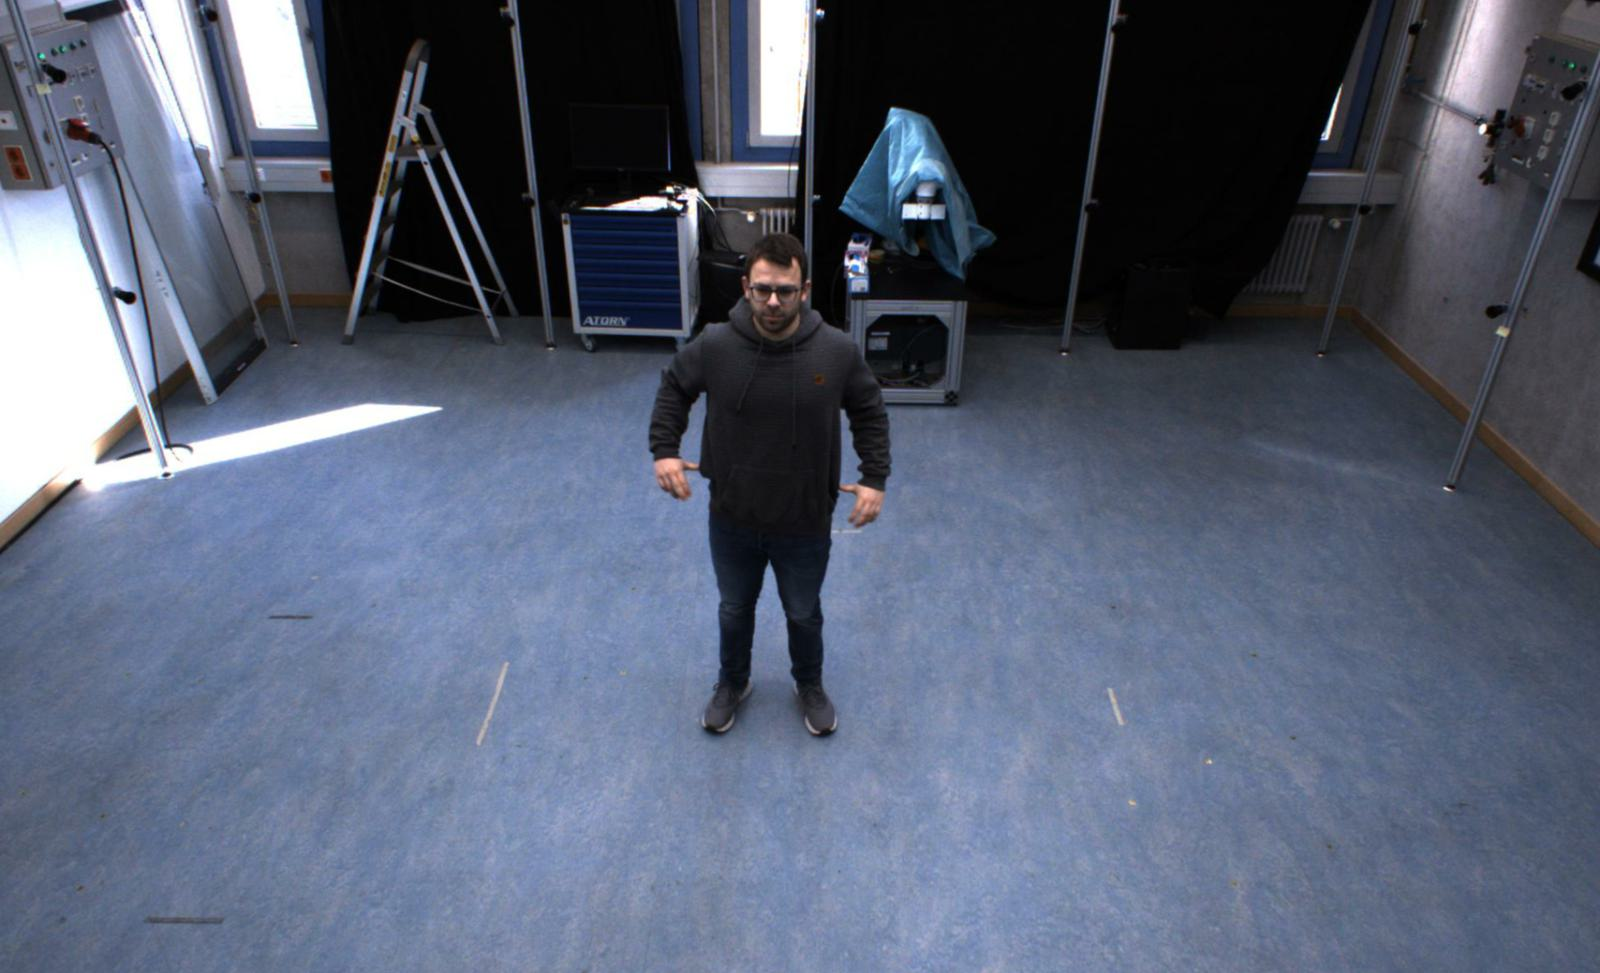
\includegraphics[width=0.48\linewidth]{bilder/Results/3dgs/3dgs_COLMAP_gt.jpg}%
    }
    \hfill
    \subfloat[Rendered Image]{%
        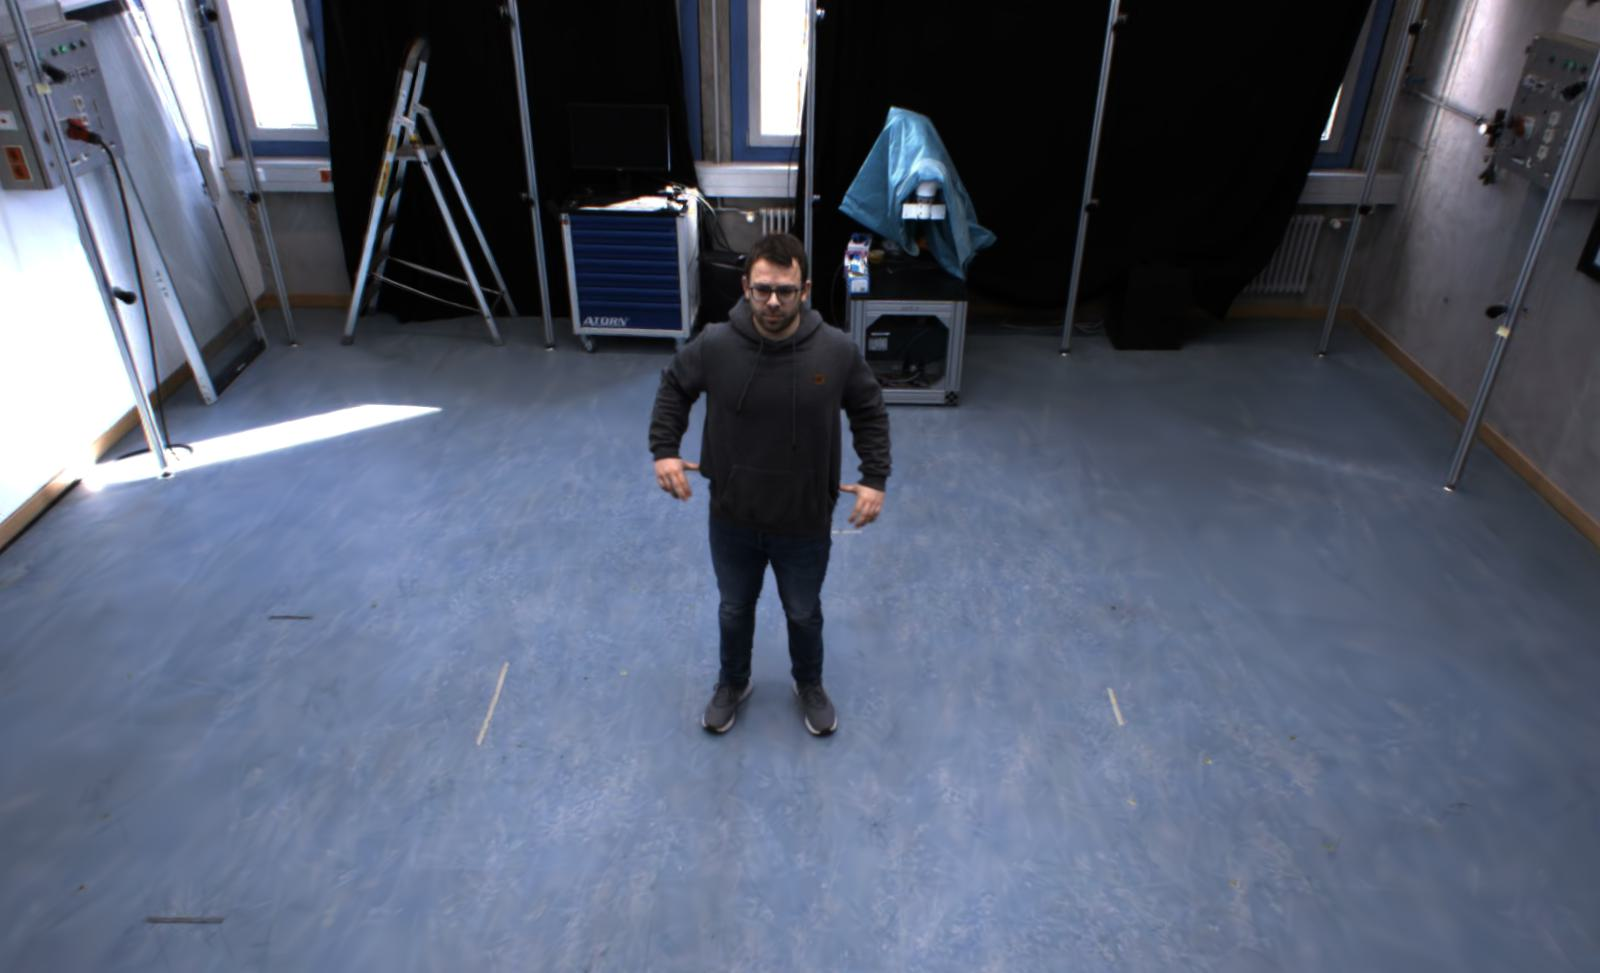
\includegraphics[width=0.48\linewidth]{bilder/Results/3dgs/3dgs_COLMAP_render.jpg}%
    }
    \caption{Comparison between ground truth and rendered image using COLMAP camera poses: The reconstruction shows clear textures in the central region, with minor blurring near the floor and image borders.}
    \label{fig:3dgs_COLMAP}
\end{figure}

\begin{figure}[h]
    \centering
    \subfloat[Ground Truth]{%
        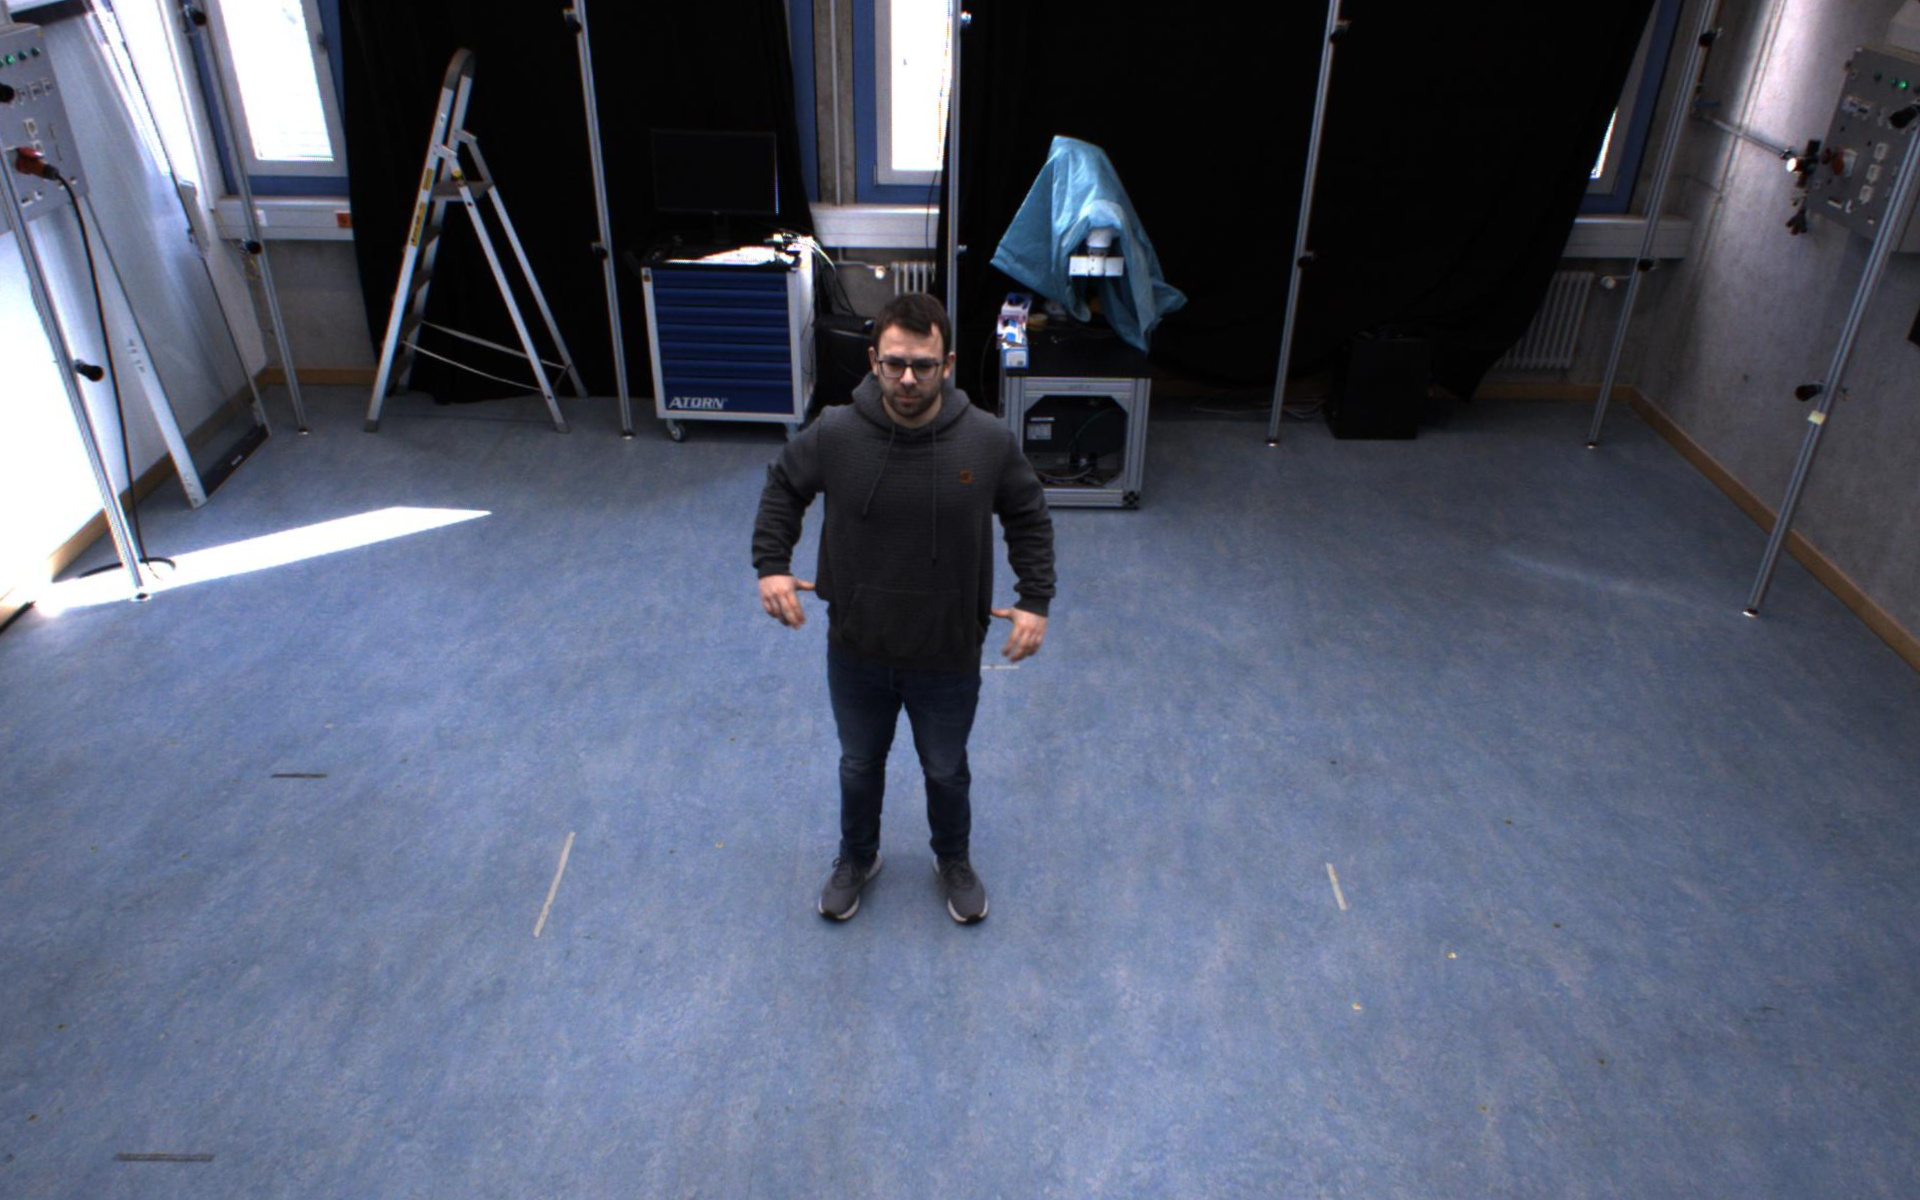
\includegraphics[width=0.48\linewidth]{bilder/Results/3dgs/3dgs_OpenCV_gt.png}%
    }
    \hfill
    \subfloat[Rendered Image]{%
        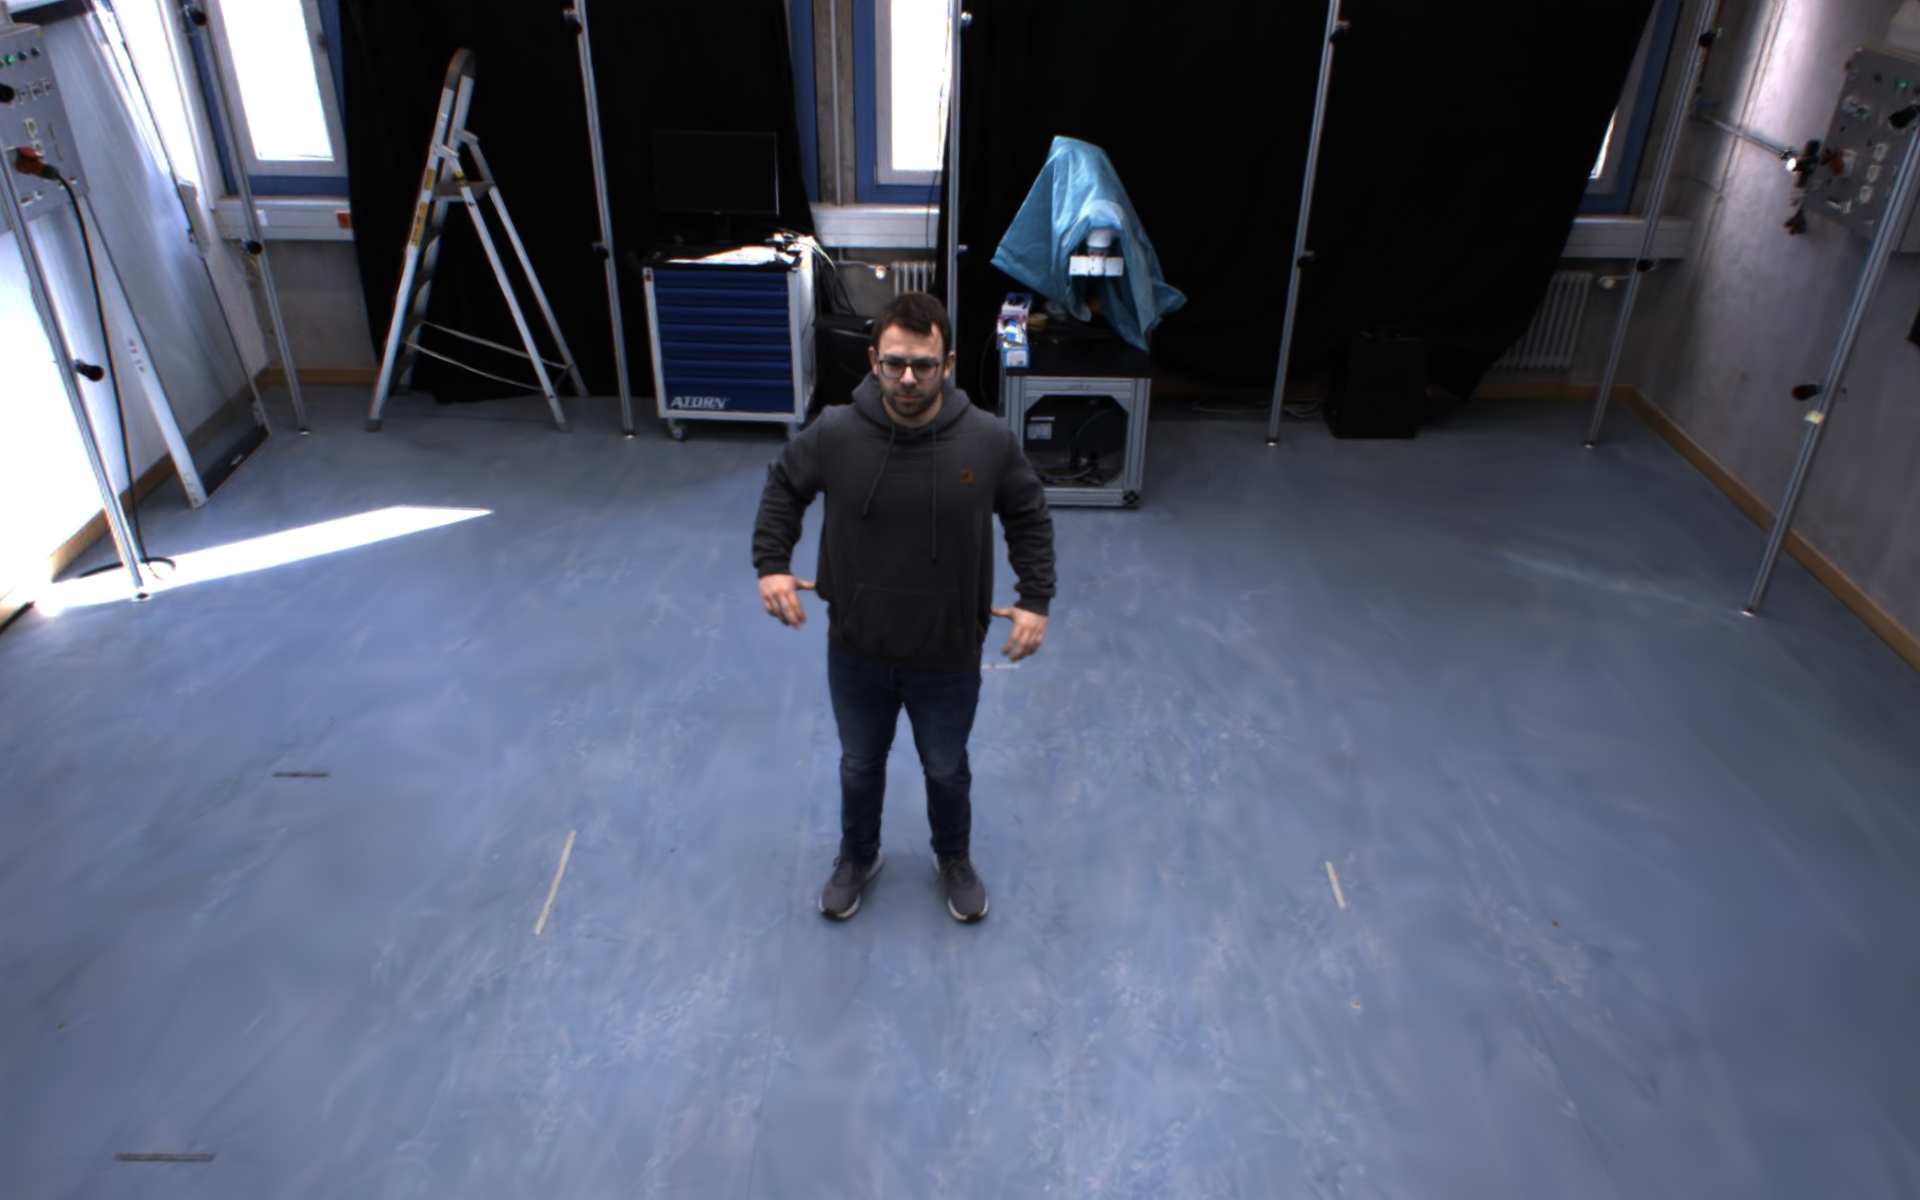
\includegraphics[width=0.48\linewidth]{bilder/Results/3dgs/3dgs_OpenCV_render.png}%
    }
    \caption{Comparison between ground truth and rendered image using OpenCV calibration: The reconstruction maintains good texture fidelity in the central region, with stronger blurring near the floor and background.}
    \label{fig:3dgs_opencv}
\end{figure}

Despite the slightly better metrics of COLMAP, OpenCV is preferred for NSTL applications, as explained in the methodology section (Chapter~\ref{chap:Methodik}). 
Deterministic calibration with OpenCV provides a coordinate system in real-world units, ensuring precise and reproducible spatial positioning. 
This is crucial for integration with other NSTL systems and for future extensions to dynamic scenes using 4D Gaussian Splatting. 
The similar reconstruction quality in the central region demonstrates that OpenCV, despite slightly lower metrics, is a robust alternative due to its consistency and lower dependence on scene-specific optimizations. 
These results provide a solid foundation for the investigation of dynamic scenes in the following sections.




\section{4D Gaussian Splatting}

\subsection{Yang et al.}

\subsubsection{Method Validation with D-NeRF and DyNeRF Datasets}
To validate the method proposed by Wang et al.~\cite{yang2023gs4d}, the D-NeRF and DyNeRF datasets were used. 
Specifically, the "Mutant" scene from the D-NeRF dataset~\cite{pumarola2021d} and the "cut roasted beef" scene from the DyNeRF dataset~\cite{li2022neural} were employed. 
Unlike the reference paper, where metrics for D-NeRF were averaged across all scenes, a scene-specific analysis was performed here. 
For DyNeRF, the reference values directly correspond to the "cut roasted beef" scene under investigation. 
The results are presented in Tables~\ref{tab:mutant_metrics} and~\ref{tab:cut_roasted_beef_metrics}. 
They show a close agreement with the reference values; deviations for D-NeRF are below 0.5~dB (PSNR) and 0.03 (SSIM), which can be attributed to the use of a single scene and slightly different training conditions. 
For DyNeRF, the implementation matches the reference values almost exactly. 

Figure~\ref{fig:mutant_comparison} illustrates the comparison between ground-truth and rendered views for the "Mutant" scene. 
The reconstructions achieve high visual consistency, with only fine details, such as the scar on the torso, appearing slightly less sharp. 

Figure~\ref{fig:DyNeRFVergleich} highlights the dependency of reconstruction quality on object motion in the "cut roasted beef" scene. 
The top row shows a frame with high object motion (knife, tongs), where blurring and partial reconstruction errors occur. 
In contrast, the bottom row depicts a frame with minimal motion, where nearly all regions are reconstructed accurately. 

\begin{table}[h]
    \centering
    \caption{Comparison of metrics for the "Mutant" scene from the D-NeRF dataset.}
    \label{tab:mutant_metrics}
    \begin{tabular}{lccc}
        \toprule
        & SSIM $\uparrow$ & PSNR (dB) $\uparrow$ & LPIPS $\downarrow$\\
        \midrule
        Reference (averaged) \cite{yang2023gs4d} & 0.98 & 34.09 & 0.02 \\
        Validation  & 0.974 & 34.135 & 0.023\\
        \bottomrule
    \end{tabular}
\end{table}

\begin{figure}[h]
    \centering
    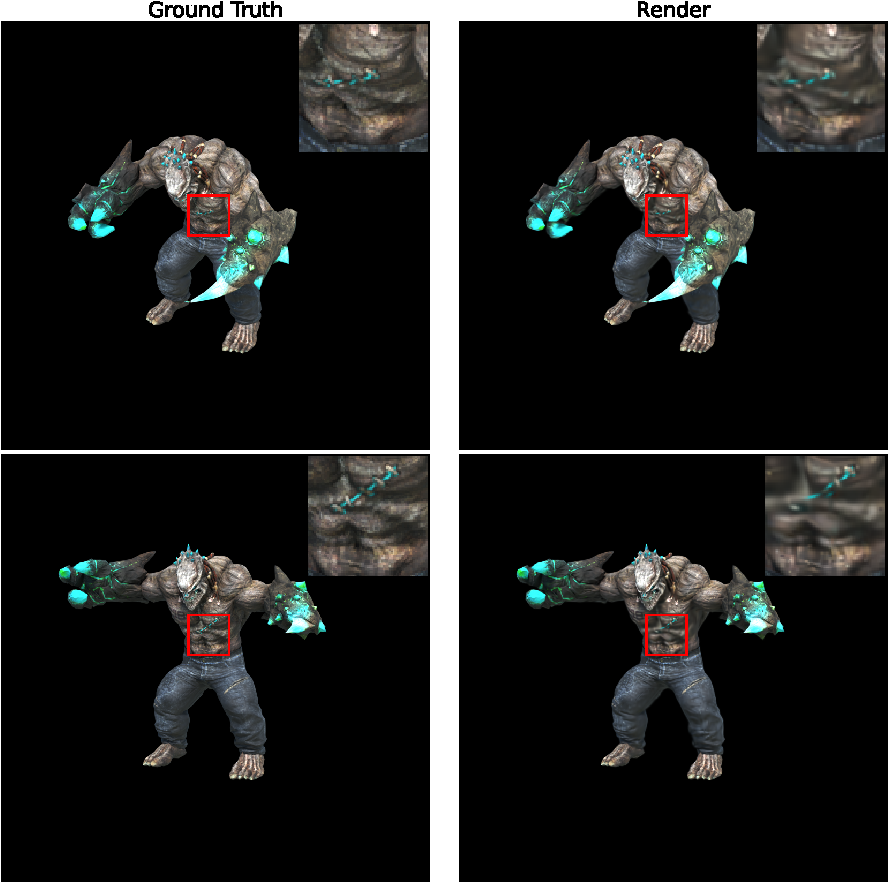
\includegraphics[width=\linewidth]{bilder/Results/Wang/DNerf/Vergleich_DNeRF.pdf}
    \caption{Example reconstruction from a test camera: While central image elements are consistently reconstructed, the ceiling exhibits strong errors due to insufficient training data coverage.}
    \label{fig:DNeRFVergleich}
\end{figure}

\begin{figure}[h]
    \centering
    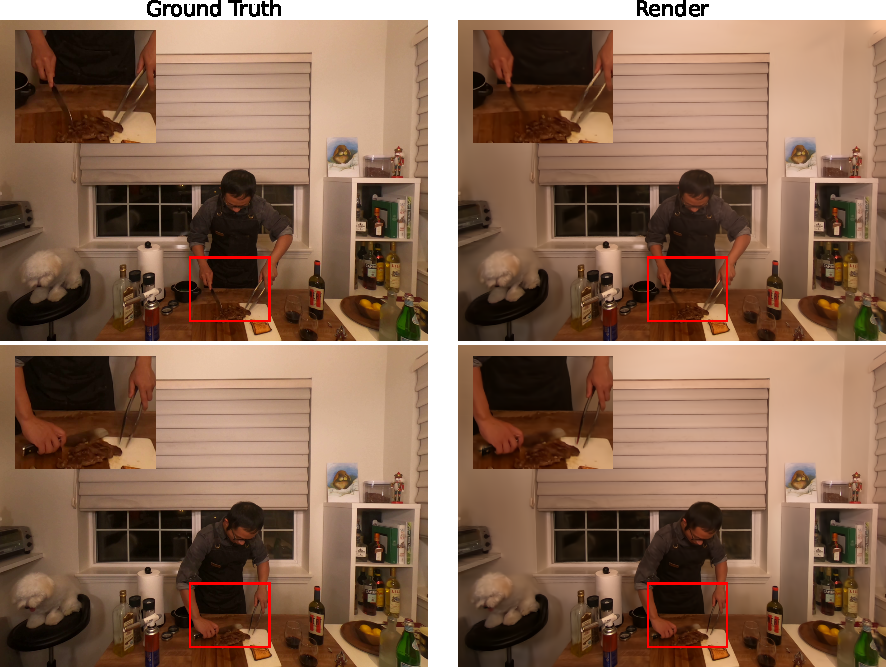
\includegraphics[width=\linewidth]{bilder/Results/Wang/DyNeRF/Vergleich_DyNeRF.pdf}
    \caption{Example reconstruction from a test camera: During high-motion frames (top), some blurring and incomplete reconstructions occur; in low-motion frames (bottom), the reconstruction quality is high across the scene.}
    \label{fig:DyNeRFVergleich}
\end{figure}

\begin{table}[h]
    \centering
    \caption{Comparison of metrics for the "cut roasted beef" scene from the DyNeRF dataset.}
    \label{tab:cut_roasted_beef_metrics}
    \begin{tabular}{lccc}
        \toprule
        & SSIM $\uparrow$ & PSNR (dB) $\uparrow$ & LPIPS $\downarrow$\\
        \midrule
        Reference \cite{yang2023gs4d} & 0.98 & 33.85 & n.a. \\
        Validation  &  0.954 & 33.163 & 0.132\\
        \bottomrule
    \end{tabular}
\end{table}

\FloatBarrier

\subsubsection{Results with the NSTL Dataset}
\label{sec:results_nstl}

Experiments with the newly captured NSTL dataset highlight the influence of the number of Gaussians on reconstruction quality. 
As shown in Table~\ref{tab:4dgs_metrics}, increasing the number of Gaussians initially leads to significant improvements, particularly from 2 million to 3.5 million Gaussians. 
The gains between 3.5 and 5 million Gaussians are less pronounced.

Figure~\ref{4dgsmodels_vs_timesteps} shows representative frames at the start and end of the sequence. 
With 2 million Gaussians, reconstruction deficiencies are evident, especially in the face and hands, which appear blurred and incomplete. 
Increasing to 3.5 million Gaussians improves facial reconstruction and clarifies hand contours, though some blurring remains. 
The 5 million Gaussian model shows no substantial improvement over the 3.5 million model, although fingers are partially reconstructed. 
Both metrics and visual inspection confirm that increasing the Gaussian count enhances reconstruction quality, particularly in fine details such as hands and fingers.

Due to memory constraints, the full sequence of 200 frames could not be trained with higher Gaussian counts. 
By reducing the sequence to 50 frames (1.6 seconds), finer modeling was possible. 
Evaluation of this shortened sequence yielded an SSIM of 0.907, a PSNR of 31.13~dB, and an LPIPS of 0.217. 
Visual comparison further supports this quality improvement. 
Figure~\ref{fig:4dgs_5mil_5e6ts} shows four representative rendered frames; the face exhibits high detail, and the hands are mostly reconstructed consistently. 
Even during overhead movements, the hands remain clear with only minor reconstruction artifacts. 

Thus, the shortened sequence significantly outperforms the full sequence (see Table~\ref{tab:4dgs_metrics}). 
The improved quality can be explained by the reduced temporal complexity, allowing more Gaussians to model fine motions, particularly in the hands.

\begin{table}[h]
    \centering
    \caption{Comparison of metrics for the NSTL "4DGS dataset" with varying numbers of Gaussians and sequence lengths.}
    \label{tab:4dgs_metrics}
    \begin{tabular}{lcccc}
        \toprule
        Sequence length & Gaussians & SSIM $\uparrow$ & PSNR (dB) $\uparrow$ & LPIPS $\downarrow$ \\
        \midrule
        200 Frames & 2M   & 0.887 & 28.67 & 0.253 \\
                   & 3.5M & 0.898 & 29.78 & 0.231 \\
                   & 5M   & 0.901 & 30.23 & 0.228 \\
        \midrule
        50 Frames  & 5M  & 0.907 & 31.13 & 0.217 \\
        \bottomrule
    \end{tabular}
\end{table}

% \begin{figure}[p]
%     \centering
%     \setlength{\tabcolsep}{4pt} % column spacing
%     \renewcommand{\arraystretch}{1.2} % row spacing
    
%     \begin{tabular}{c c c c}
%         & \textbf{t = 0}  & \textbf{t = 199} \\

%         \rotatebox{90}{\textbf{GT}} &
%         \includegraphics[width=0.48\textwidth]{bilder/Results/Wang/GT_C-1-M_000000.jpg} &
%         \includegraphics[width=0.48\textwidth]{bilder/Results/Wang/GT_C-1-M_000199.jpg} \\

%         \rotatebox{90}{\textbf{2M}} &
%         \includegraphics[width=0.48\textwidth]{bilder/Results/Wang/2_mil_pts_C-1-M_000000.jpg} &
%         \includegraphics[width=0.48\textwidth]{bilder/Results/Wang/2_mil_pts_C-1-M_000199.jpg} \\
        
%         \rotatebox{90}{\textbf{3.5M}} &
%         \includegraphics[width=0.48\textwidth]{bilder/Results/Wang/3.5_mil_pts_C-1-M_000000.jpg} &
%         \includegraphics[width=0.48\textwidth]{bilder/Results/Wang/3.5_mil_pts_C-1-M_000199.jpg} \\

%         \rotatebox{90}{\textbf{5M}} &
%         \includegraphics[width=0.48\textwidth]{bilder/Results/Wang/5_mil_pts_C-1-M_000000.jpg} &
%         \includegraphics[width=0.48\textwidth]{bilder/Results/Wang/5_mil_pts_C-1-M000199.jpg} \\

%     \end{tabular}

%     \caption{Comparison of models (rows) and timesteps (columns).}
%     \label{fig:4dgsmodels_vs_timesteps}
% \end{figure}


\begin{figure}[h]
    \centering
    \includegraphics[width=\linewidth]{bilder/Results/Wang/4D Tennis/50img/Vergleich_Volley_50img.pdf}
    \caption{Comparison of ground truth (left) and rendered images (right) for the 4D Tennis dataset with 50 images.}
    \label{fig:DyNeRFVergleich}
\end{figure}


\FloatBarrier





\subsubsection{Results of the Pruning Approach}
\label{pruning_results}

The experiments show that the proposed pruning approach can significantly reduce the model's memory footprint without substantially compromising image quality. 
Compared to the previous best model with 5M Gaussians (9.6~GB memory), the number of Gaussians could be reduced by up to 70\%. 
At the same time, evaluation metrics improved slightly (see Table~\ref{tab:4dgs_metrics}). 

The model with pruning applied after densification (1.5M Gaussians) already shows a notable improvement over the baseline. 
Further integration of pruning during densification (1.8M Gaussians) led to additional metric gains. 
This indicates that short-lived and redundant Gaussians are indeed removed early and replaced with more relevant ones. 

Visual comparisons (Fig.~\ref{fig:4dgs_prune}) present a more nuanced picture. 
While global metrics suggest improvements, Gaussians are also removed in critical areas such as the fingers. 
Pruning after densification shows some improvement in the fingers, whereas pruning during densification results in reduced quality in fingertip modeling. 
This highlights that metrics capture visual quality only partially, as they emphasize improvements in static regions over losses in dynamic regions, which occupy less spatial area.  

\paragraph{Analysis of Active Gaussians}  

Notably, the number of active Gaussians per timestep increases significantly due to pruning (from ~20\% to over 35\%), as shown in Fig.~\ref{fig:Pruning_overview} (a). 
Rendering times are also reduced because fewer Gaussians need to be projected onto the 2D image plane. 
Covariance values, however, change only slightly, indicating that the temporal persistence of individual Gaussians is minimally affected by pruning (see Fig.~\ref{fig:Pruning_overview} (b)). 
This may also be related to the scene complexity. 
Unlike DyNeRF scenes, NSTL recordings contain large-scale movements. 
To capture detailed hand motions, Gaussians with low covariance are required to model fine-grained movements.

These results illustrate a fundamental trade-off of the pruning approach: 
While reducing the number of Gaussians and the associated memory savings leads to significantly improved quantitative metrics, qualitative results show deterioration in areas with complex motion, such as the hands. 
Metrics primarily benefit from sharper reconstructions of static backgrounds, whereas dynamic details lose precision due to the removal of relevant Gaussians. 
This suggests that pruning strategies, although promising for efficiency, should be complemented by adaptive methods that evaluate each Gaussian not only for persistence but also in the context of dynamic motion. 
Such an approach could achieve a better balance between memory usage, numerical metrics, and perceived visual quality in the long term.

\begin{table}[h]
    \centering
    \caption{Comparison of metrics for the NSTL "4DGS dataset" with varying Gaussian counts and memory usage.}
    \label{tab:4dgs_metrics}
    \begin{tabular}{ccccc}
        \toprule
        Number of Gaussians & Memory (Gb) & SSIM $\uparrow$ & PSNR (dB) $\uparrow$ & LPIPS $\downarrow$ \\
        \midrule
        5M   & 9.6 & 0.907 & 31.13 & 0.217 \\
        1.5M & 2.9 & 0.926 & 32.83 & 0.164 \\
        1.8M & 3.5 & 0.940 & 33.12 & 0.133 \\
        \bottomrule
    \end{tabular}
\end{table}

\begin{figure}
    \centering
    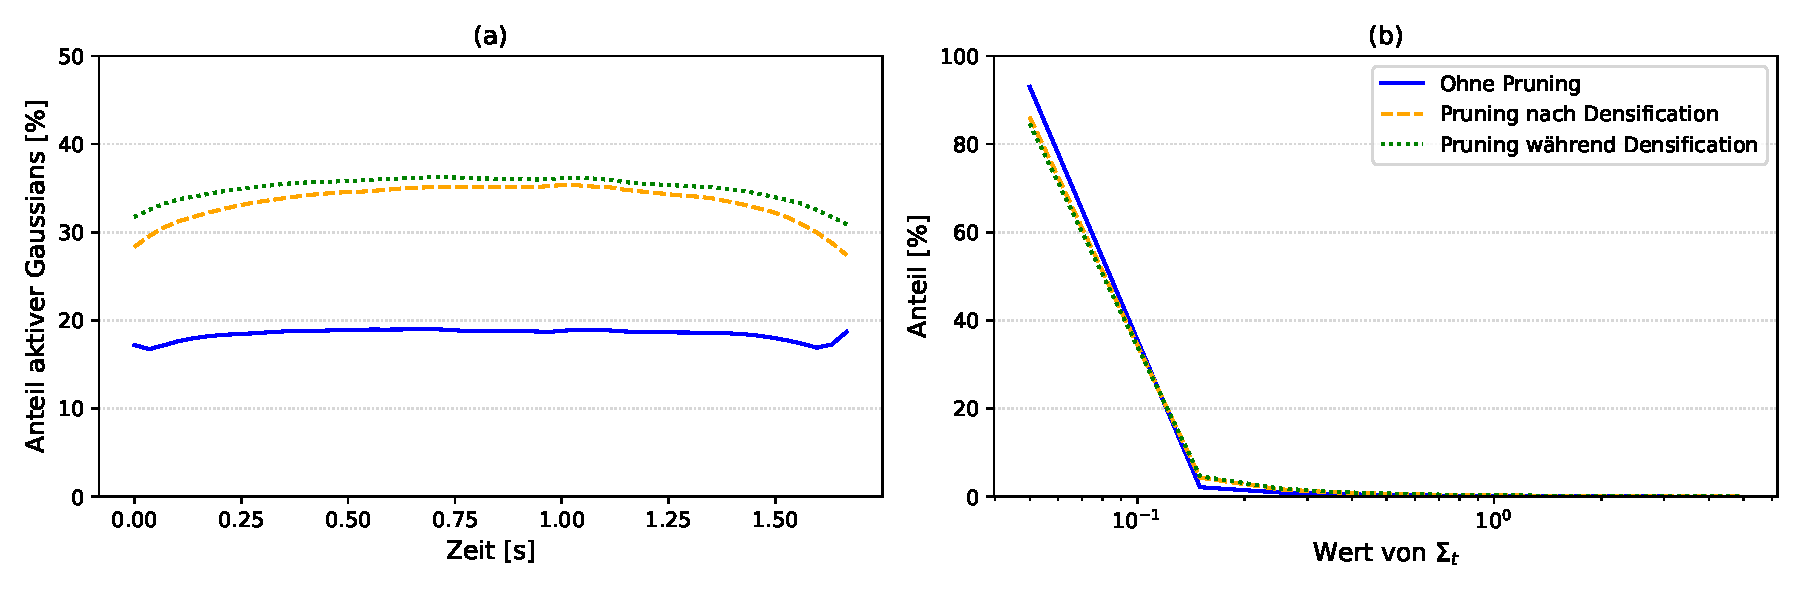
\includegraphics[width=1\linewidth]{bilder//Results//Wang//Prune/Overview_Pruning.pdf}
    \caption{Comparison of different pruning strategies: 
    (a) proportion of active Gaussians over time, 
    (b) distribution of $\Sigma_t$.}
    \label{fig:Pruning_overview}
\end{figure}

\begin{figure}[htbp]
    \centering

    % --- Row 1 ---
    \begin{minipage}[b]{0.48\textwidth}
        \centering
        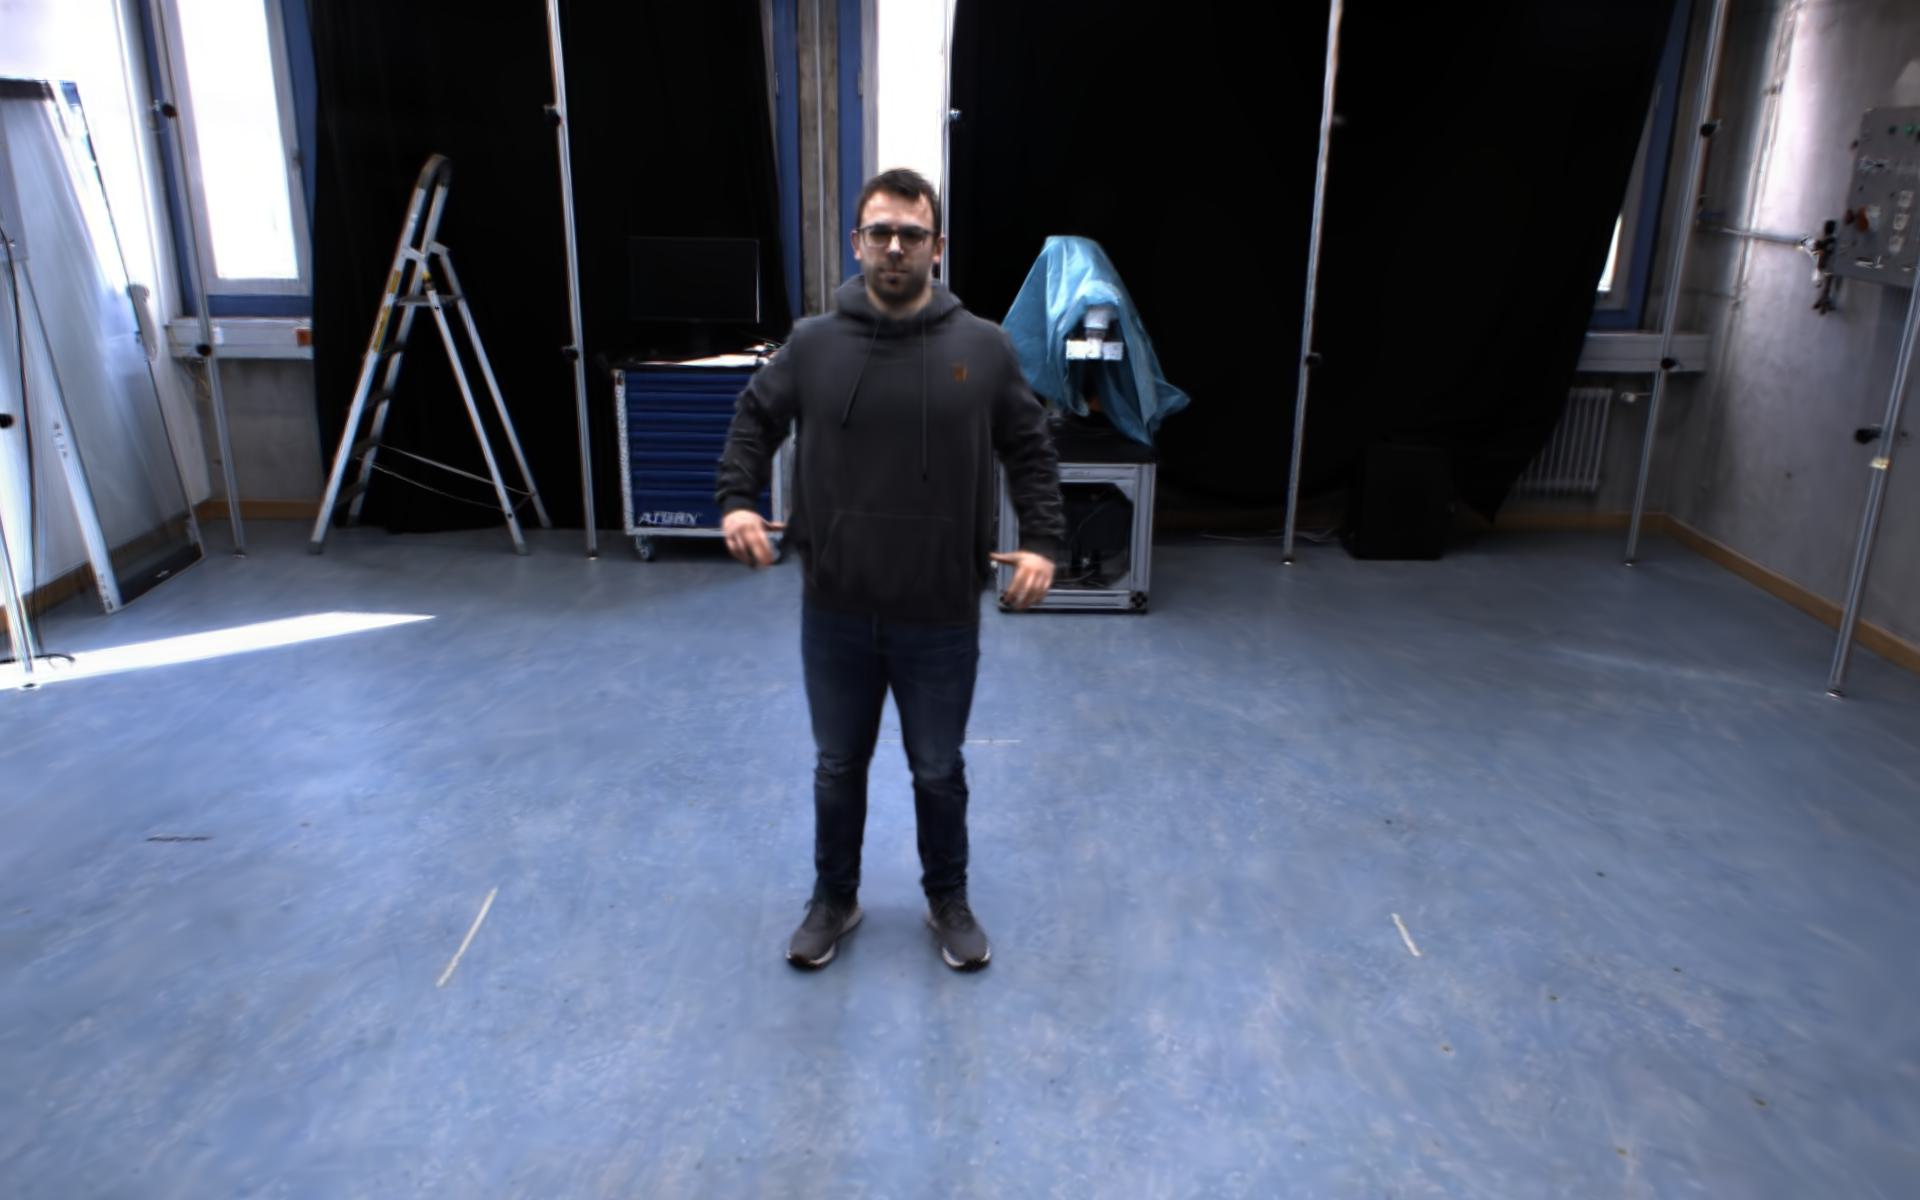
\includegraphics[width=\linewidth]{bilder/Results/Wang/Prune/C-1-M_000000.jpg}
        \caption*{(a) Ground Truth 1}
    \end{minipage}\hfill
    \begin{minipage}[b]{0.48\textwidth}
        \centering
        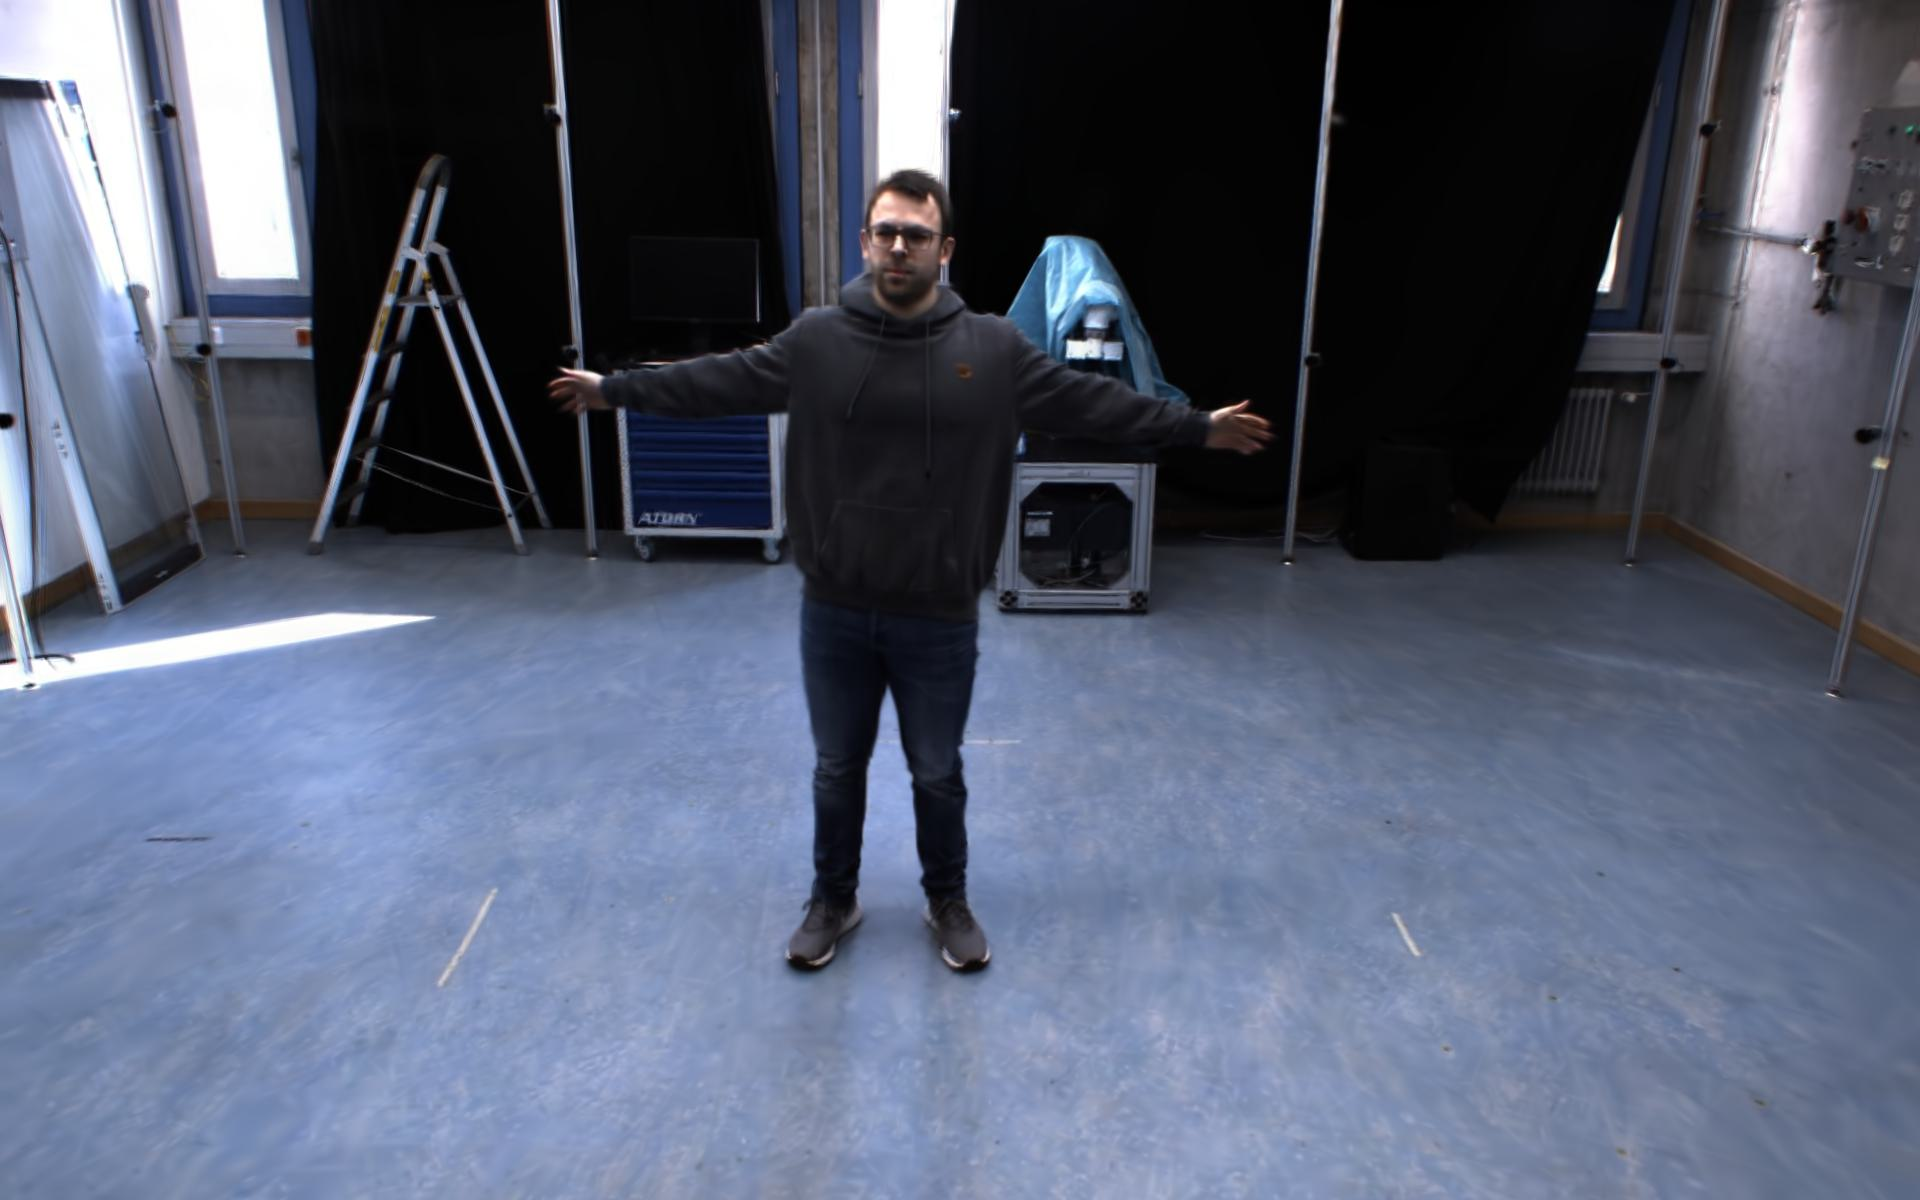
\includegraphics[width=\linewidth]{bilder/Results/Wang/Prune/C-1-M_000015.jpg}
        \caption*{(b) Render 1 (Pruning during Densification)}
    \end{minipage}

    \vspace{0.5cm}

    % --- Row 2 ---
    \begin{minipage}[b]{0.48\textwidth}
        \centering
        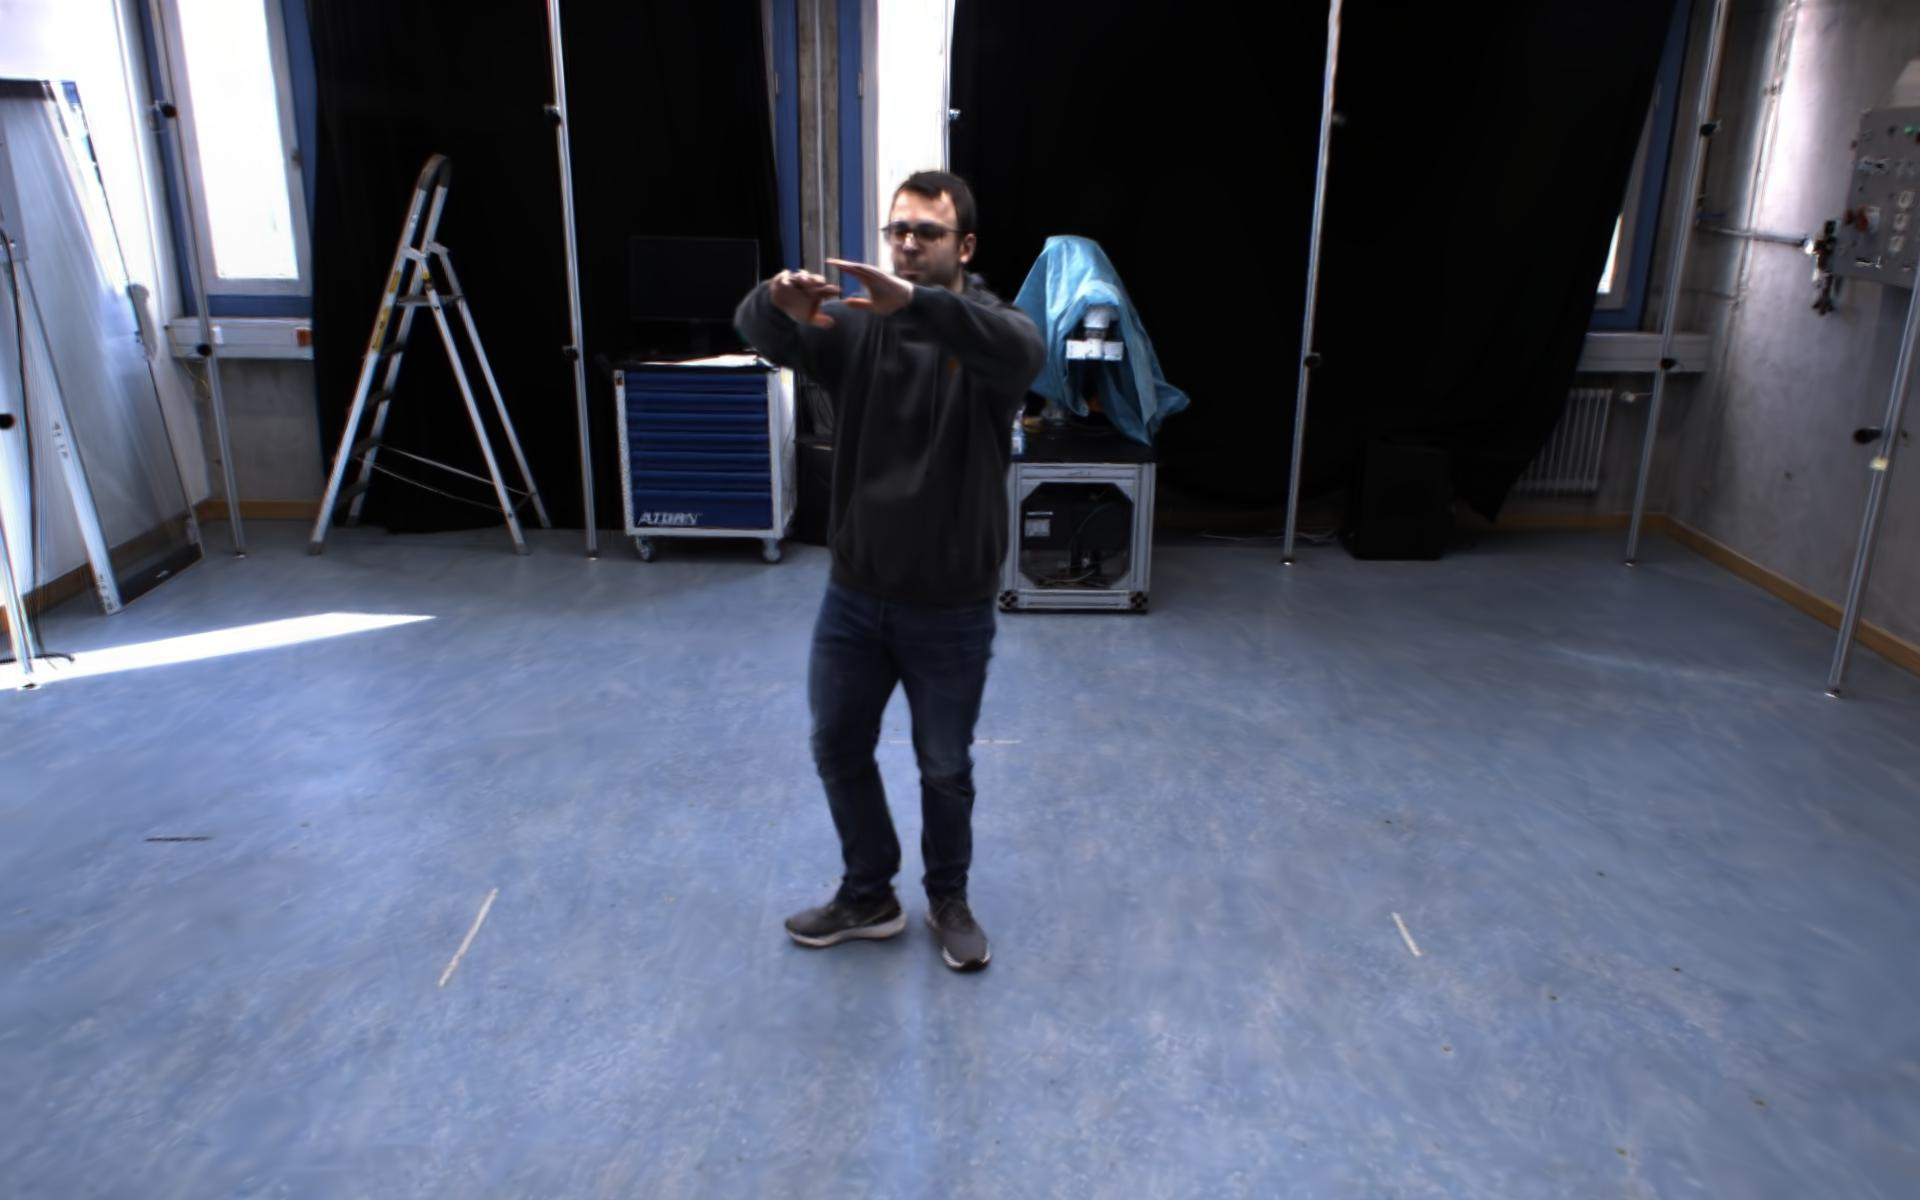
\includegraphics[width=\linewidth]{bilder/Results/Wang/Prune/C-1-M_000030.jpg}
        \caption*{(c) Ground Truth 2}
    \end{minipage}\hfill
    \begin{minipage}[b]{0.48\textwidth}
        \centering
        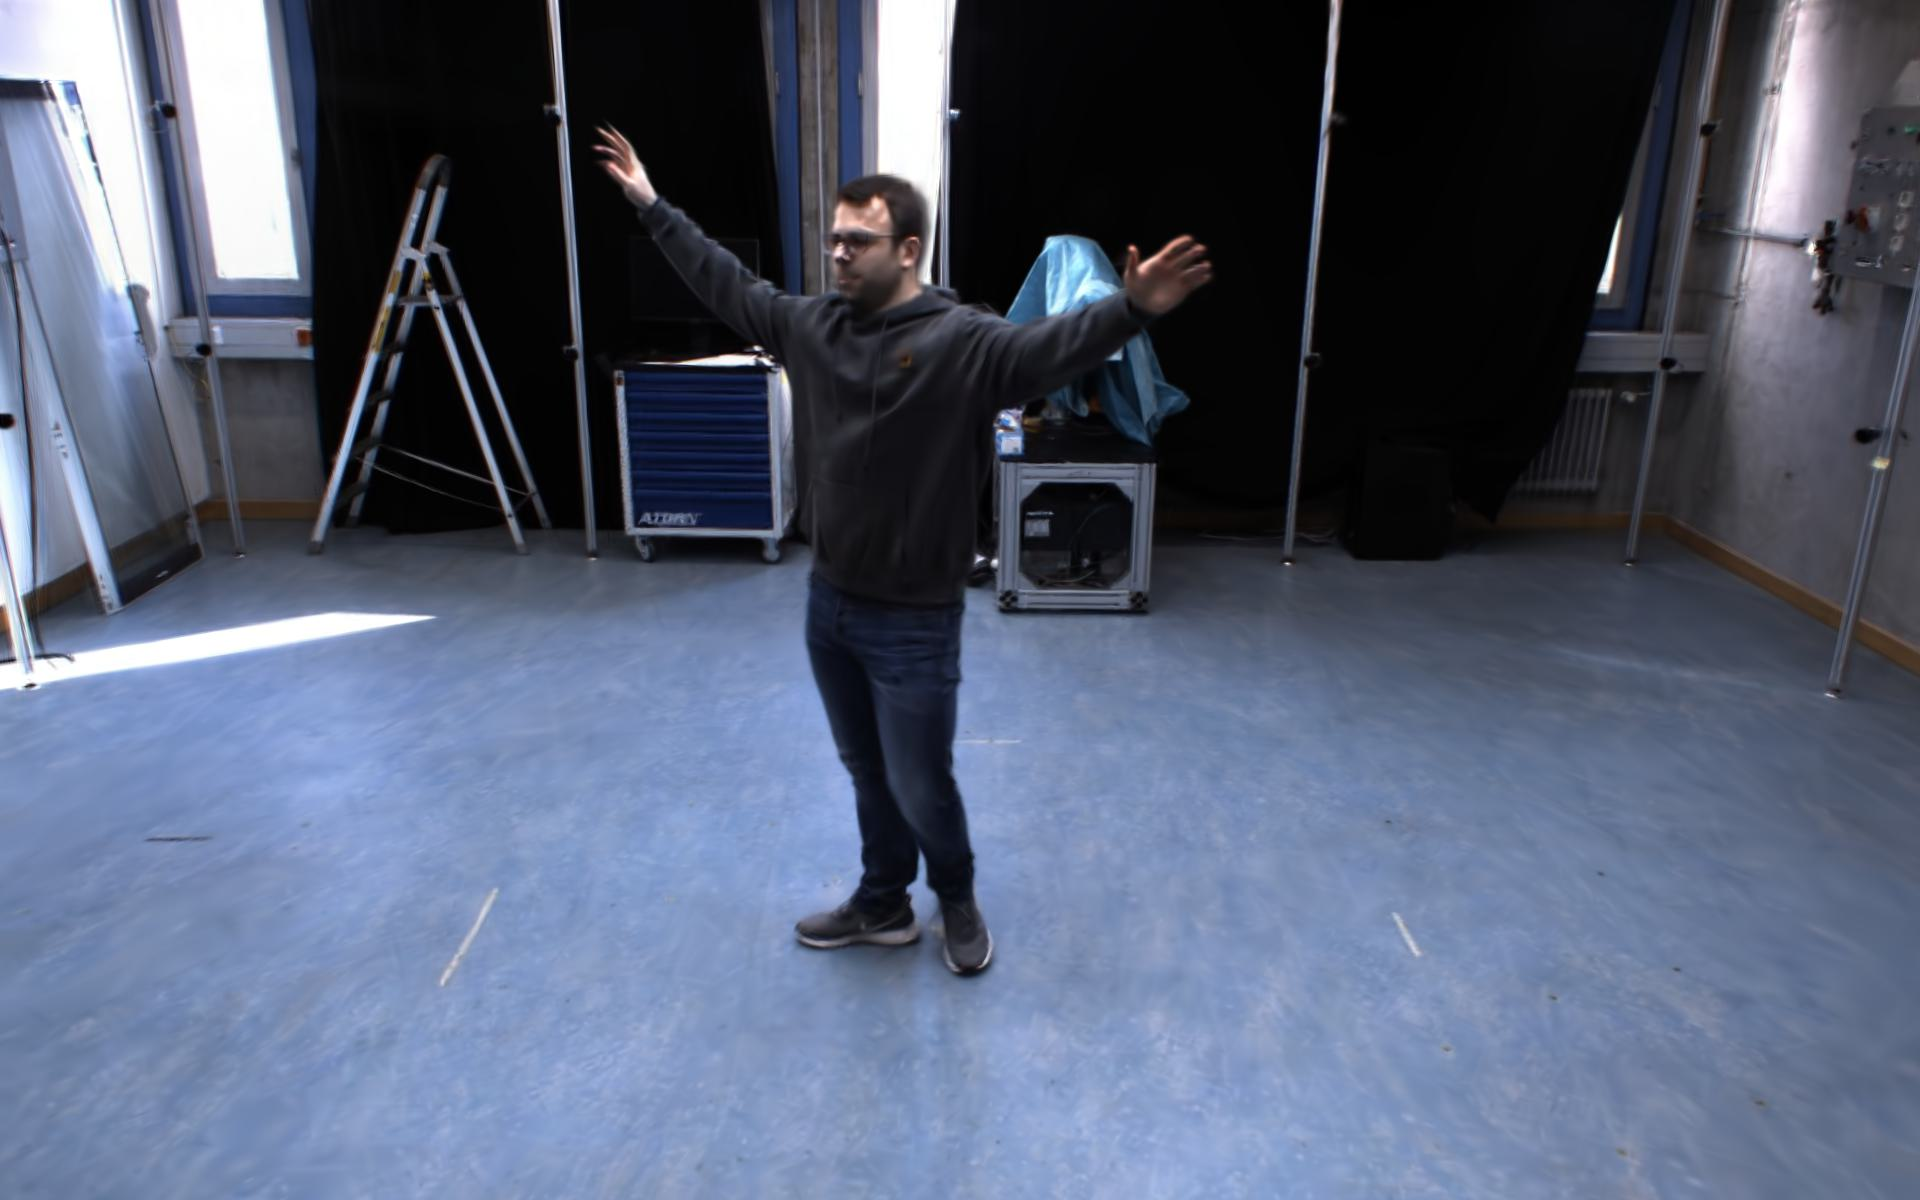
\includegraphics[width=\linewidth]{bilder/Results/Wang/Prune/C-1-M_000040.jpg}
        \caption*{(d) Render 2 (Pruning during Densification)}
    \end{minipage}

    \caption{Comparison of ground truth (left) and rendered images (right) for camera C-1-M. 
    While background details improve with pruning, foreground regions (hands) exhibit qualitative weaknesses.}
    \label{fig:4dgs_prune}
\end{figure}

\FloatBarrier

\subsection{Volley Dataset}

Experiments show that capturing a cleaned-up scene already results in a significant improvement (see Table~\ref{tab:4dgs_clean_metrics}). 
Without explicit pruning, the total number of Gaussians reduced to 3.7M (7.1~GB), while quality metrics increased significantly compared to the original 5M Gaussian scene.

\begin{table}[h]
    \centering
    \caption{Comparison of metrics between the original and cleaned scene.}
    \label{tab:4dgs_clean_metrics}
    \begin{tabular}{ccccc}
        \toprule
        Scene & Number of Gaussians & SSIM $\uparrow$ & PSNR (dB) $\uparrow$ & LPIPS $\downarrow$ \\
        \midrule
        Original & 5M   & 0.907 & 31.13 & 0.217 \\
        Cleaned  & 3.7M & 0.937 & 35.8  & 0.159 \\
        \bottomrule
    \end{tabular}
\end{table}

Qualitative results (Fig.~\ref{fig:4dgs_clean}) confirm the numerical improvements. 
The scene is reconstructed more sharply and consistently, especially in static regions previously burdened by unnecessary background Gaussians. 
Global player movements are modeled accurately in most frames. 

However, a closer analysis reveals a more nuanced picture. 
While early frames are nearly perfectly aligned with ground truth, the swing motion shows initial limitations. 
The light green stripes on the racket appear blurred and lose detail, obscuring sharp edges. 
This indicates that modeling fast movements and fine structures remains challenging. 
On the positive side, the hand without the racket is reconstructed much more consistently and with more detail compared to previous experiments. 
This demonstrates a key advantage of the cleaned scene: model capacity is focused on relevant objects and motions. 
Moreover, the number of Gaussians was not limited by memory during training, as the 5M maximum capacity was not reached. 
Observed limitations are therefore due to the challenge of representing fast movements with high fidelity rather than model size constraints.

Overall, these experiments show that careful selection of a cleaned scene can achieve substantial improvements without complex pruning strategies. 
Previous results indicated that redundant Gaussians negatively affect memory and quality; the new scene confirms this observation under realistic conditions.

\begin{figure}
    \centering
    \includegraphics[width=1\linewidth]{bilder//Results//Wang//4D Tennis//50img/Vergleich_Volley_50img.pdf}
    \caption{placeholder}
    \label{fig:4DTennis50img_GtvsRender}
\end{figure}

\subsection{Training with Fixed Background}

Integrating a fixed background into the training process leverages the specific structure of the NSTL setup. 
Before the start of a sequence, a reference image of the empty scene can be captured from each camera, so that static scene elements are represented directly via these background images rather than Gaussians. 
This allows the model capacity to focus on dynamic objects.

Results from training with 50 images show that this approach yields high-quality reconstructions. 
Both the racket surface and the player’s hands are modeled with sharp edges and consistent geometry throughout the sequence. 
In contrast, training with 300 images leads to increased reconstruction errors, particularly blurring of the hands, face, and fine structures on the racket.

Numerical evaluation with PSNR, SSIM, or LPIPS is not meaningful in this scenario. 
Since the background is explicitly embedded via reference images and not modeled with Gaussians, reconstructed background areas appear largely black in the renderings. 
This distorts metrics, which would not reflect the quality of dynamic reconstruction. 
Instead, renderings reveal isolated bright Gaussians on the floor. 
These artifacts are due to inconsistencies between static and dynamic captures, especially shadows present only during motion that are absent in the reference image.

The degradation with 300 images can be attributed to increased optimization complexity. 
With six times more training images, both the number of Gaussians to be placed and the diversity of scene content increases, leading to reduced model capacity for focusing on fine details in individual regions.











\section{Composition Pipeline Evaluation}

This chapter presents a qualitative evaluation of the proposed multi-camera compositing and dynamic scene generation pipeline. 
In the absence of complete ground-truth annotations, the analysis focuses on visual consistency, temporal coherence, and scene-level generalization across multiple reconstruction and rendering configurations. 
All results were produced using the same calibrated multi-camera rig under identical rendering parameters, without manual post-processing unless explicitly stated.

\section{Compositional Scene Generation}
Figure~\ref{fig:composition} illustrates how the proposed compositing pipeline integrates multiple independently reconstructed Gaussian Splatting models into a single, globally aligned scene. 
Each row in the figure shows one configuration step, starting from a single-object placement and progressing toward increasingly populated scenes that combine both static and dynamic objects.
For each configuration, the corresponding RGB renderings, depth maps, bounding boxes, and segmentation overlays are presented to demonstrate multi-modal coherence.

A central advantage of the system is that all semantic annotations, including instance masks, class indices, and bounding boxes, are generated automatically and remain geometrically consistent across all rendered views. 
Since every 3D model is represented as Gaussian primitives within a shared coordinate system, mask generation requires no additional training or inference using segmentation networks. 
All semantic labels are deterministically derived from the compositing process itself, ensuring reproducible and noise-free annotations.

The modular design of the pipeline further enables high scene variability. 
Objects can be translated, rotated, scaled, or duplicated directly in 3D space without retraining or manual re-annotation. 
This flexibility allows large-scale dataset creation with controlled variation in object arrangement and spatial relationships. 
In practice, the same set of Gaussian models can be reused across numerous novel compositions while preserving consistent geometry, color, and semantic labeling, making the approach well suited for scalable and reproducible synthetic dataset generation.

\begin{figure*}[t]
    \centering
    \includegraphics[width=\textwidth]{Grafiken/Composition.pdf}
    \caption{
        \textbf{Compositional scene generation.}
        Example of multi-object scenes composed from independently reconstructed Gaussian Splatting models. 
        Each row shows one scene configuration with RGB, depth, bounding boxes, and segmentation overlays.
        All semantic annotations are generated automatically and remain spatially consistent across views.
    }
    \label{fig:composition}
\end{figure*}

\section{Multi-view Occlusion Handling}
To assess the robustness of the compositing mechanism under occlusions, 
Figure~\ref{fig:occlusion} shows segmentation overlays from two viewpoints of a scene containing interacting dynamic subjects. 
Even when large parts of one subject are occluded, the instance masks remain spatially consistent and tightly aligned with visible contours. 
This demonstrates that the rendering process preserves correct inter-object depth ordering and instance integrity across multiple perspectives. 
Such behavior is crucial for generating reliable training data for tasks such as instance segmentation or 3D scene understanding, where stable occlusion boundaries are essential.

\begin{figure}[ht]
    \centering
    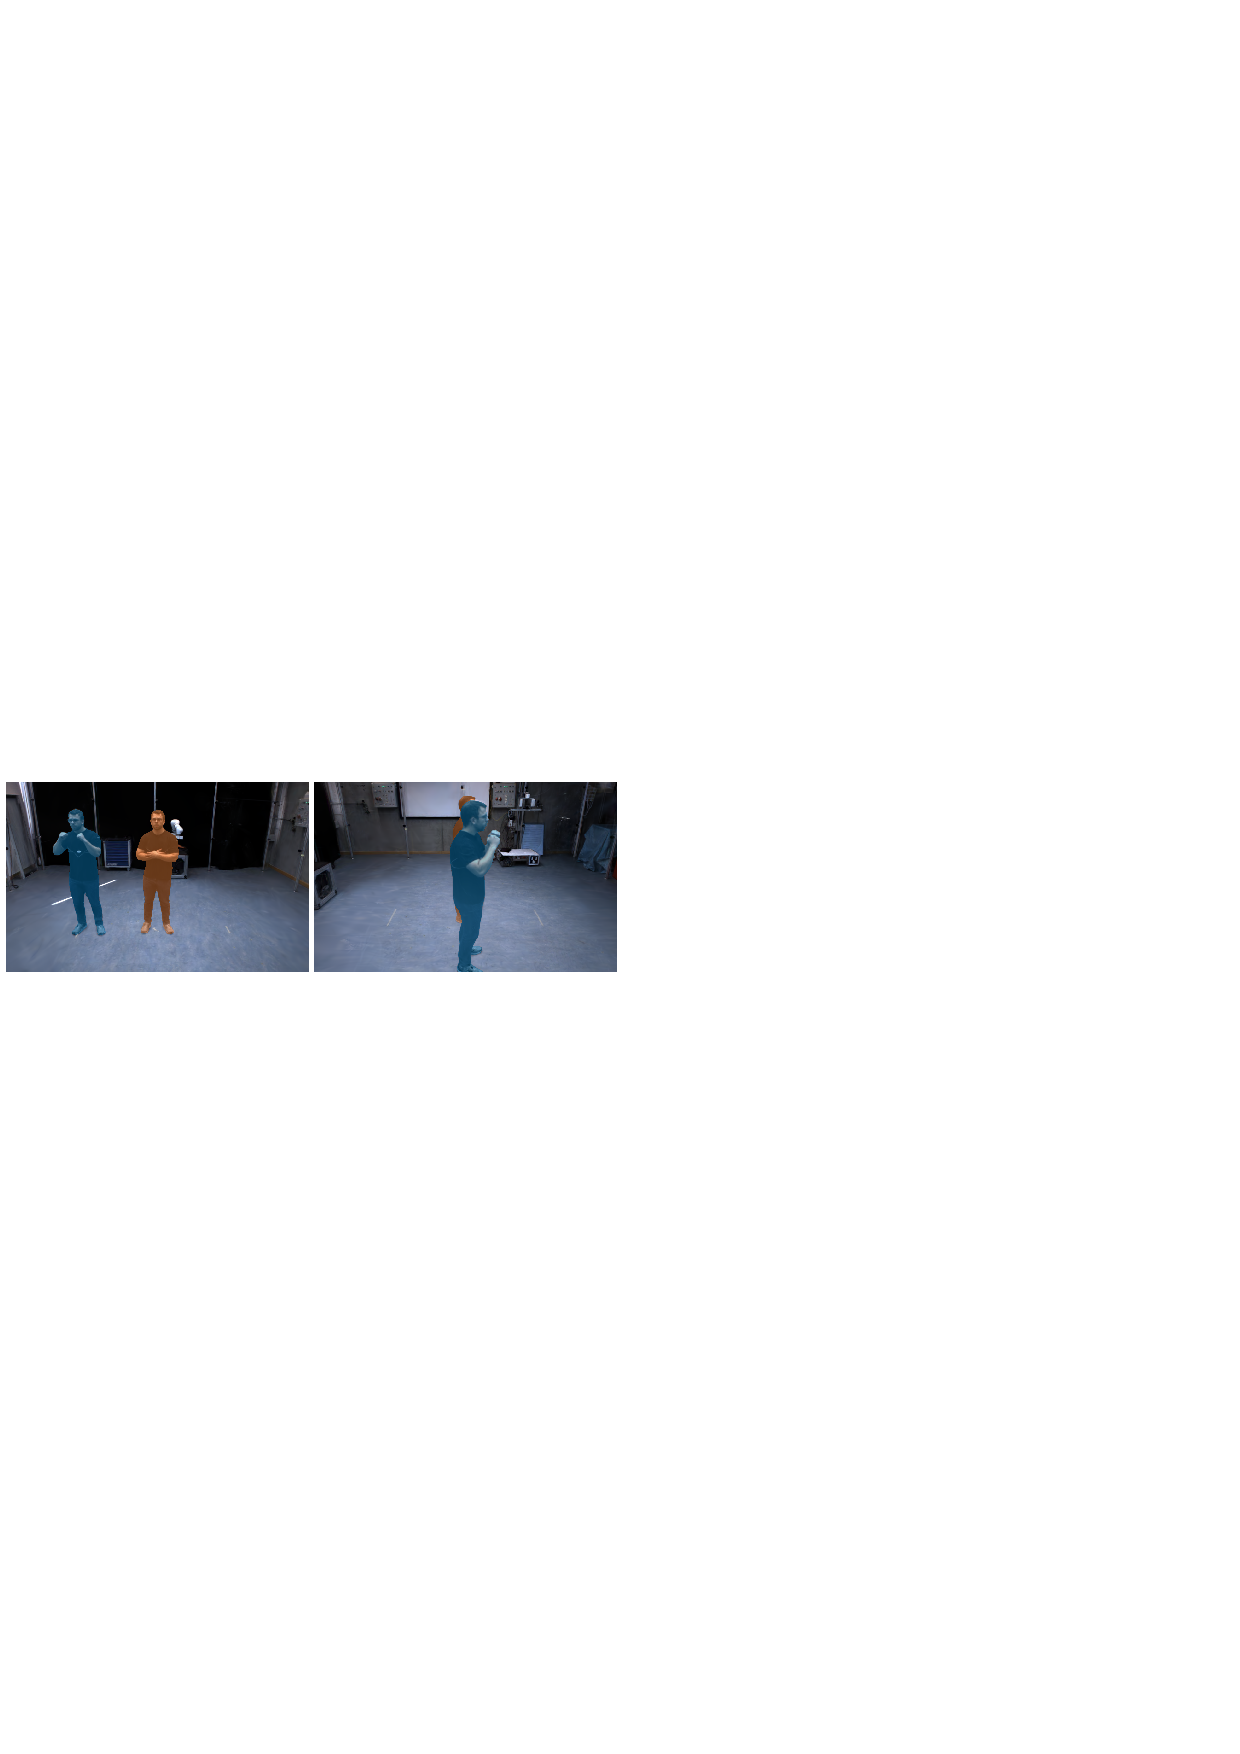
\includegraphics[width=\linewidth]{Grafiken/Oclusion.pdf}
    \caption{
        \textbf{Occlusion handling across views.}
        Segmentation overlays from front and side viewpoints of two interacting subjects.
        Even under strong mutual occlusion, instance masks remain consistent and well aligned with visible contours.
    }
    \label{fig:occlusion}
\end{figure}

\section{Scene Generalization}
Figure~\ref{fig:generalization} demonstrates the adaptability of the proposed system by recontextualizing dynamic subjects within a novel virtual environment reconstructed from real imagery using COLMAP \cite{schoenberger2016sfm}. 
The reconstructed environment provides realistic geometry and camera poses that serve as a spatial reference for compositing. 
Dynamic subjects are seamlessly integrated into the new setting, maintaining correct spatial alignment, depth consistency, and segmentation coherence. 
By decoupling object-level Gaussian models from a specific environment, the system enables arbitrary recombination of dynamic and static assets across scenes without retraining. 
This generalization capability supports large-scale variation in scene composition and facilitates applications such as domain adaptation, robustness evaluation, and synthetic-to-real transfer.

\begin{figure}[ht]
    \centering
    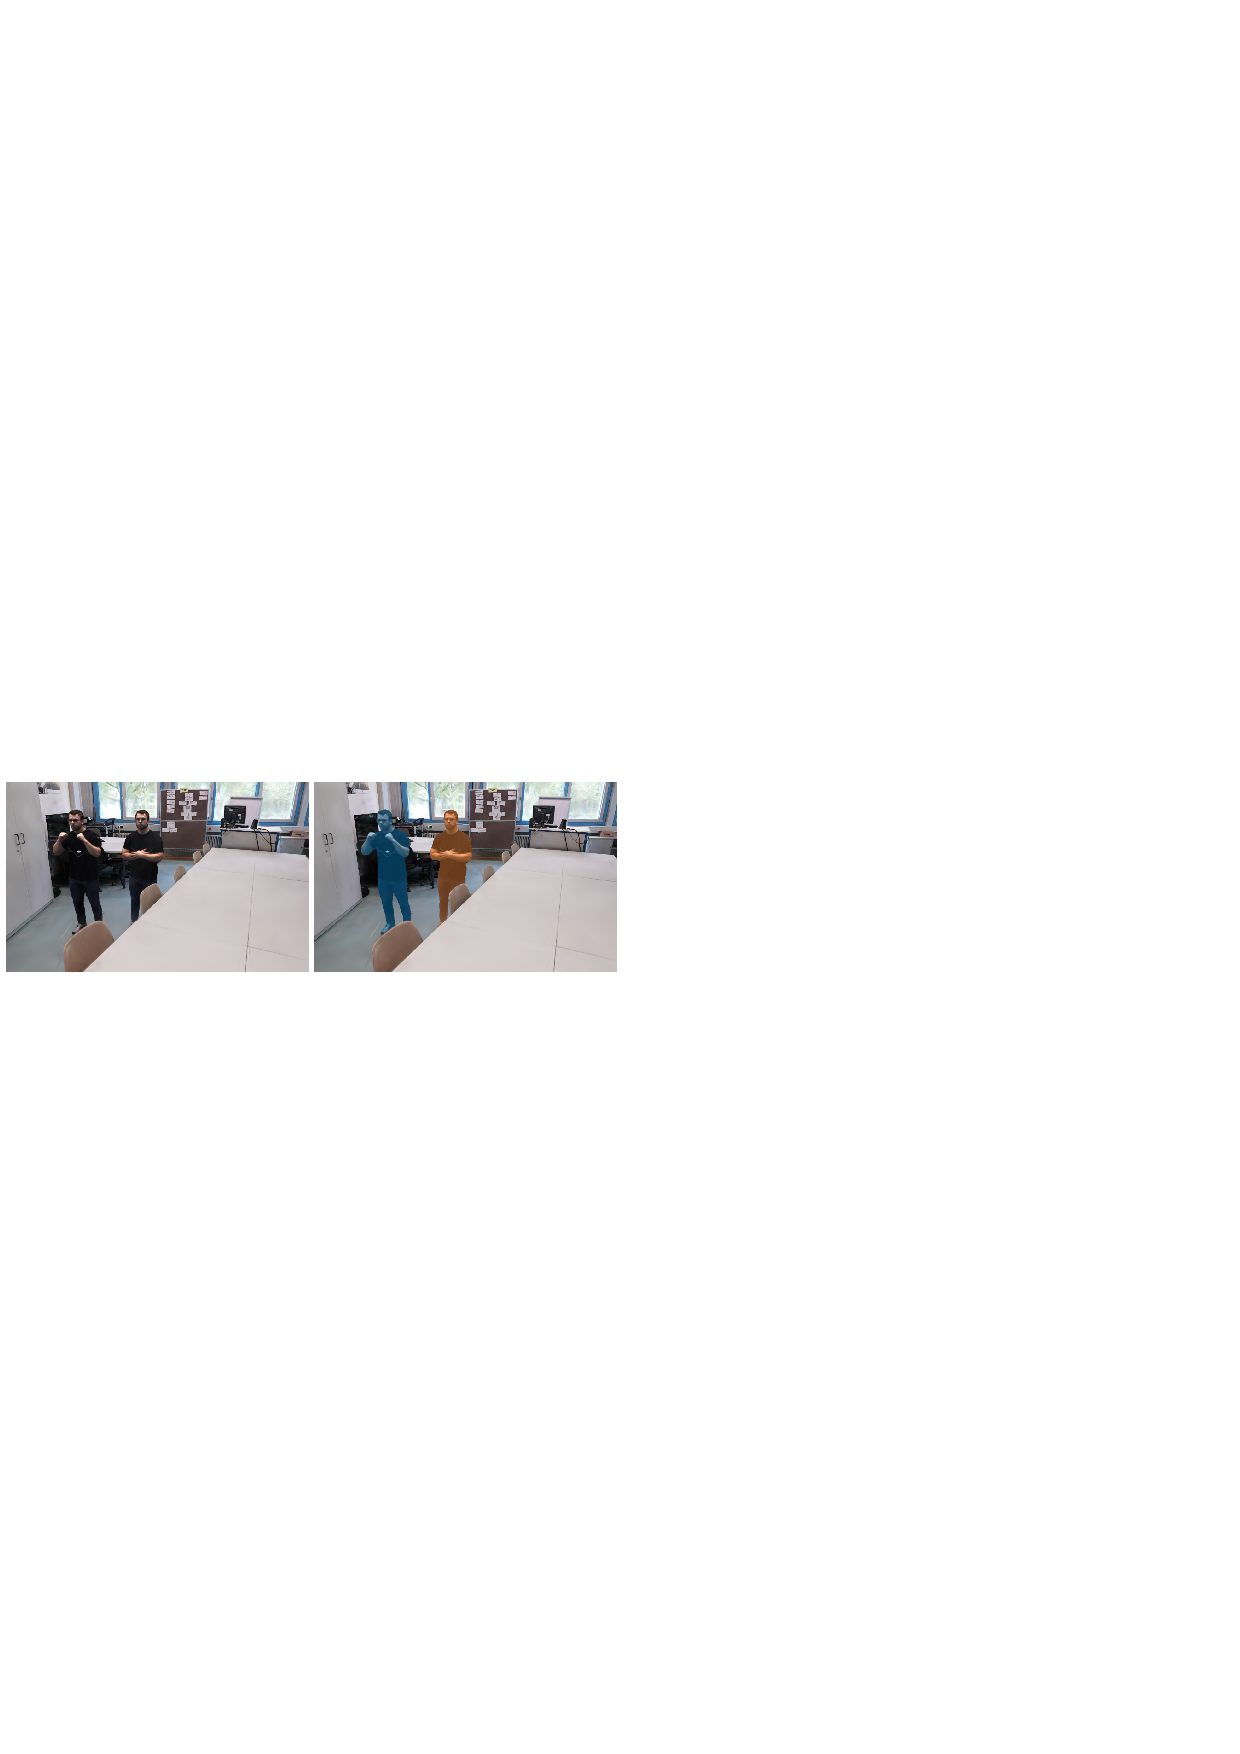
\includegraphics[width=\linewidth]{Grafiken/room_transfer.pdf}
    \caption{
        \textbf{Scene generalization and recontextualization.}
        Dynamic subjects composited into a novel virtual environment reconstructed with COLMAP.
        The system maintains consistent geometry and segmentation alignment across domains, 
        demonstrating flexible recontextualization of pre-trained Gaussian models.
    }
    \label{fig:generalization}
\end{figure}

\section{Temporal Consistency in Dynamic Scenes}
Dynamic scene rendering enables the generation of temporally coherent 4D datasets suitable for applications such as activity recognition, pose estimation, or motion segmentation. 
Figure~\ref{fig:temporal} shows representative frames from a dynamic sequence of a moving subject. 
The RGB and segmentation overlays reveal smooth and consistent motion over time, with stable geometry and accurate alignment across frames. 
Each time step preserves object structure and surface continuity, indicating that the Gaussian-based transformation updates produce interpretable and stable temporal behavior. 
This capability allows scalable synthesis of realistic dynamic sequences without requiring explicit motion capture or manual supervision.

\begin{figure*}[t]
    \centering
    \includegraphics[width=\textwidth]{Grafiken/time.pdf}
    \caption{
        \textbf{Dynamic scene generation.}
        Representative time steps of a moving subject with RGB and segmentation overlays.
        The consistent motion and geometry across frames demonstrate temporally stable 4D rendering.
    }
    \label{fig:temporal}
\end{figure*}

\section{Qualitative Pose Estimation}
Figure~\ref{fig:keypoints} (top row) shows qualitative 6D pose estimates for a dynamic human sequence across four time steps. 
Each frame visualizes the canonical object coordinate system derived from the aggregated Gaussian transformations. 
Although no ground-truth pose data are available, the estimated coordinate axes evolve consistently and reflect plausible orientation changes relative to the subject’s motion. 
This indicates that Gaussian-based transformation tracking provides a reliable approximation of object-level motion, suitable for downstream tasks such as pose refinement or motion analysis.

\section{Keypoint Propagation}
The lower row of Figure~\ref{fig:keypoints} visualizes the temporal keypoint propagation results obtained with a Detectron2-based detector \cite{Detectron22020}. 
Initial 2D keypoints are detected in a reference frame and projected into 3D by associating them with the nearest Gaussian centroids of the corresponding subject. 
As a result, keypoints are anchored on the object surface rather than the true anatomical joints, but they remain spatially coherent throughout the sequence. 
The keypoints are subsequently propagated in time according to the motion of the underlying Gaussians.

Temporal stability is observed across most body regions, particularly in the upper body where Gaussian density is high and motion is well captured. 
Minor deviations appear in areas with sparse or unstable Gaussian coverage, such as the knees or hips, leading to small temporal inconsistencies or spatial offsets. 
Despite these limitations, the propagation maintains overall semantic coherence and demonstrates that the Gaussian-based motion field can sustain meaningful correspondences over time. 
This behavior provides a promising foundation for future integration with articulated motion priors or learned joint-space constraints.

\begin{figure*}[t]
    \centering
    \includegraphics[width=\textwidth]{Grafiken/keypoints.pdf}
    \caption{
        \textbf{Qualitative analysis of pose and keypoint propagation.}
        Four frames of a dynamic subject showing estimated object poses (top) and propagated keypoints (bottom).
        The coordinate systems evolve consistently over time, while keypoint trajectories remain coherent despite local misalignments.
    }
    \label{fig:keypoints}
\end{figure*}

% \section{Summary}
% Overall, these qualitative results highlight that our framework can produce temporally stable geometric and semantic representations for dynamic scenes. 
% Although both pose and keypoint estimation currently rely on unsupervised tracking without ground-truth reference, the observed consistency across time demonstrates the potential of our 4D Gaussian representation as a foundation for future work in motion analysis, activity recognition, and articulated model learning.



